\section{La compression JPEG}
Le format \textbf{JPEG (Joint Photographic Experts Group)} est un format d'image très utilisé. Contrairement aux formats d'image tels que PNG ou BMP qui sont des formats sans perte,
JPEG utilise une compression avec perte similaire à la transformée de Fourier discrète appelée \textbf{Transformée en cosinus discrète (DCT)}. 
La compression JPEG repose sur la décomposition de l'image en blocs carrés.
Chaque bloc est décomposé en une somme de cosinus de fréquences différentes. Le spectre ainsi obtenu peut alors être compressé en ne gardant que les fréquences les plus faibles.
Il ne reste alors qu'à faire la transformation inverse (analogue à la transformée de Fourier inverse) et de rassembler les blocs pour obtenir une image compressée.

\subsection{Transformée en Cosinus Discrète (DCT)}
La \textbf{Transformée en Cosinus Discrète (DCT)} est une transformation linéaire orthogonale qui projette un vecteur réel 
$x = (x_0, x_1, \dots, x_{N-1}) \in \mathbb{R}^N$ sur une base de fonctions cosinus. Elle est largement utilisée en traitement du signal et en compression d'images.

La DCT-II, qui est la plus couramment utilisée, est définie par :
$$X_k = \sum_{n=0}^{N-1}x_n\cos \left[\frac{\pi}{N}\left(n+\frac{1}{2}\right)k\right], \qquad k = 0,1,...,N-1$$

Pour obtenir une transformation orthonormée, on ajoute des facteurs de normalisation :
$$X_k = \alpha_k\sum_{n=0}^{N-1}x_n\cos \left[\frac{\pi}{N}\left(n+\frac{1}{2}\right)k\right]$$
avec 
$$\alpha_k = \left\{ 
    \begin{array}{cl}\sqrt{\frac{1}{N}} \quad \text{si } k=0 
    \\\sqrt{\frac{2}{N}} \quad \text{si } k \ge 1 
\end{array} \right.$$

On définit les fonctions de base de la DCT :
$$ e_k(n) = \alpha_k \cos\left(\frac{\pi}{N}\left(n+\frac{1}{2}\right)k\right),\quad k=0,\dots,N-1 $$

Les $(e_k)$ forment une base orthonormale pour le produit scalaire usuel sur $\mathbb{R}^N$.

\begin{proof}
    On considère le produit scalaire usuel sur $\mathbb{R}^N$ :
    $ \langle x,y\rangle = \sum_{n=0}^{N-1} x_ny_n $
    On calcule :
    \begin{align*}
        \langle e_k,e_l\rangle 
        &= \alpha_k \alpha_l \sum_{n=0}^{N-1} \cos\left(\frac{\pi}{N}\left(n+\frac{1}{2}\right)k\right) \cos\left(\frac{\pi}{N}\left(n+\frac{1}{2}\right)l\right)\\
        \text{On peut remarquer que }&\sum_{n=0}^{N-1} \cos\left(\theta\left(n + \frac{1}{2}\right)\right) = \frac{\sin(N\theta/2)}{2\sin(\theta)}\\
        \langle e_k,e_l\rangle
        &= \frac{\alpha_k \alpha_l}{2} \left( \frac{\sin(N(\theta_k - \theta_l))}{2\sin((\theta_k - \theta_l)/2)} + \frac{\sin(N(\theta_k + \theta_l))}{2\sin((\theta_k + \theta_l)/2)} \right) \\
        &= \frac{\alpha_k \alpha_l}{4} \left( \frac{\sin(\pi(k-l))}{\sin(\pi(k-l)/2N)} + \frac{\sin(\pi(k+l))}{\sin(\pi(k+l)/2N)} \right)
    \end{align*}
\begin{itemize}
    \item Si $k \neq l \implies \langle e_k,e_l\rangle = \sin(\pi(k-l)) = \sin(\pi(k+l)) = 0$
    \item Si $k=l \neq 0$, le premier terme vaut $2N$ et le second est nul :
    $\langle e_k,e_k\rangle = \frac{\alpha_k^2}{4} 2N = \frac{1}{2N}2N= 1$
    \item Si $k=l=0$, les deux termes vaut $2N$ par continuité en 0 :
    $\langle e_0,e_0\rangle = \frac{\alpha_0^2}{4} (2N + 2N) = 1$
\end{itemize}

    Ainsi, la famille $(e_k)$ forme une base orthonormale de $\mathbb{R}^N$.
\end{proof}



La DCT peut être vue comme une décomposition du signal sur une base orthogonale de cosinus de fréquences croissantes. 
L'avantage de ne pas utiliser des sinus comme avec la transformée de Fourier est que les valeurs retournées restent réelles. \\

La DCT possède plusieurs propriétés importantes :
\begin{itemize}
    \item \textbf{Linéarité} : la transformation est linéaire.
    \item \textbf{Orthogonalité} : les vecteurs sont orthogonaux.
    \item \textbf{Energie concentrée} : l'énergie du signal est concentrée dans un petit nombre de coefficients.
    \item \textbf{Inverse} : il existe une transformée inverse (IDCT) permettant de reconstruire exactement le signal initial
\end{itemize}

L'orthogonalité est un atout important de cette transformation car elle permet de conserver l'énergie d'un signal. \\
En effet, si on note $ E = \sum_{n=0}^{N-1} x_n^2= \norm{x}^2$ l'énergie du signal $x = (x_0,...,x_{N-1})$ et $A$ la matrice orthogonale associée à cette transformation alors : \\
\begin{align*}
    \norm{X}^2 &= X^tX = (Ax)^t(Ax) = x^tA^tAx \\
               &= x^tx = \norm{x}^2
\end{align*}
Cette propriété assure donc qu'il n'y a pas de perte d'information après la transformation. Ainsi, on peut appliquer une transformation inverse afin de retrouver le signal original.
 La transformée inverse, notée IDCT est :
$$x_n = \sum_{k=1}^{N-1}\alpha_k X_k\cos \left[\frac{\pi}{N}\left(n+\frac{1}{2}\right)k\right], \qquad k = 0,1,...,N-1$$
On a alors IDCT(DCT($x_n$)) = $x_n$
\begin{proof}
    \begin{align*}
        X_k = \alpha_k\sum_{m=0}^{N-1}x_m\cos \left[\frac{\pi}{N}\left(m+\frac{1}{2}\right)k\right] \\
        x_n = \sum_{k=0}^{N-1}\alpha_k X_k\cos \left[\frac{\pi}{N}\left(n+\frac{1}{2}\right)k\right]\\
        IDCT(DCT(x_n))&=\sum_{k=0}^{N-1}\alpha_k \left(\alpha_k\sum_{m=0}^{N-1}x_m\cos \left[\frac{\pi}{N}\left(m+\frac{1}{2}\right)k\right]\right)\cos \left[\frac{\pi}{N}\left(n+\frac{1}{2}\right)k\right]\\
                      &=\sum_{k=0}^{N-1}\left(\alpha_k^2\sum_{m=0}^{N-1}x_m\cos \left[\frac{\pi}{N}\left(m+\frac{1}{2}\right)k\right]\right)\cos \left[\frac{\pi}{N}\left(n+\frac{1}{2}\right)k\right]\\
                      &=\sum_{m=0}^{N-1}x_m\left(\sum_{k=0}^{N-1}\alpha_k^2\cos \left[\frac{\pi}{N}\left(m+\frac{1}{2}\right)k\right]\cos \left[\frac{\pi}{N}\left(n+\frac{1}{2}\right)k\right]\right)\\
                      &=\sum_{m=0}^{N-1}x_m\left(\sum_{k=0}^{N-1}\left(\alpha_k\cos \left[\frac{\pi}{N}\left(m+\frac{1}{2}\right)k\right]\right)\left(\alpha_k\cos \left[\frac{\pi}{N}\left(n+\frac{1}{2}\right)k\right]\right)\right) \\
        \text{Posons }e_i(k)&=\alpha_k\cos\left[\frac{\pi}{N}\left(i+\frac{1}{2}\right)k\right], e_i=(e_i(0),e_i(1),...,e_i(N-1)) \in \mathbb{R}^N \\
                      &=\sum_{m=0}^{N-1}x_m\left(\sum_{k=0}^{N-1}e_m(k)e_n(k)\right) \\
                      &=\sum_{m=0}^{N-1}x_m\langle e_m,e_n\rangle =\sum_{m=0}^{N-1}x_m\delta_{m,n} = x_n
    \end{align*}
\end{proof}

\subsection{Transformation en blocs}
Le format JPEG divise les images en blocs de pixels (de taille $8 \times 8$ dans notre implémentation). On peut alors appliquer la DCT sur chacun des blocs. 
Cette découpe est avantageuse car les pixels au sein d'un même bloc sont souvent corrélés. De plus, il existe des implémentations efficaces permettant d'éviter des calculs répétifs. 
On peut alors calculer les coefficients en cosinus une seule fois :

$$(C_1, C_2, C_3, C_4, C_5, C_6, C_7)
=\sqrt{\frac{2}{N}} \cdot\left(\cos\frac{\pi}{16}, \cos\frac{2\pi}{16}, \cos\frac{3\pi}{16}, \cos\frac{4\pi}{16},
 \cos\frac{5\pi}{16}, \cos\frac{6\pi}{16}, \cos\frac{7\pi}{16}\right)$$

Une optimisation possible est l'utilisation de la propriété de symétrie du cosinus. \\
Commençons par poser $$ \theta_{n,k} \coloneq \frac{\pi}{8}(n+\frac{1}{2})k $$ \\
Remarquons que  $$\theta_{7-n,k} = \frac{\pi}{8}(7-n+\frac{1}{2})k = \frac{\pi}{8}(\frac{15}{2}-n)k $$
Ainsi $$x_{7-n}cos(\theta_{7-n,k}) = x_{7-n}(-1)^kcos(\theta_{n,k}) = \pi k- \theta_{n,k} $$\\
On peut alors utiliser cette propriété pour réduire le nombre de calculs à effectuer.
\begin{align*}
    X_k &= \alpha_k\sum_{n=0}^7[x_n\cos(\theta_{n,k})]\\
    &= \alpha_k\sum_{n=0}^3[x_n\cos(\theta_{n,k})+x_{7-n}\cos(\theta_{7-n,k})] \\
    X_k &= \alpha_k\sum_{n=0}^3[x_n+(-1)^kx_{7-n}]cos(\theta_{n,k})
\end{align*}


On obtient alors les $X_k$ à l'aide des multiplications matricielles : 
$$\begin{pmatrix} X_0 \\ X_2 \\ X_4 \\ X_6 \end{pmatrix}
=
\begin{pmatrix}
C_4 & C_4 & C_4 & C_4 \\
C_2 & C_6 & -C_6 & -C_2 \\
C_4 & -C_4 & -C_4 & C_4 \\
C_6 & -C_2 & C_2 & -C_6
\end{pmatrix}
\cdot
\begin{pmatrix} x_0 + x_7 \\ x_1 + x_6 \\ x_2 + x_5 \\ x_3 + x_4 \end{pmatrix}$$

$$\begin{pmatrix} X_1 \\ X_3 \\ X_5 \\ X_7\end{pmatrix}
=
\begin{pmatrix}
C_1 & C_3 & C_5 & C_7 \\
C_3 & -C_7 & -C_1 & -C_5 \\
C_5 & -C_1 & C_7 & C_3 \\
C_7 & -C_5 & C_3 & -C_1
\end{pmatrix}
\cdot
\begin{pmatrix} x_0 - x_7 \\ x_1 - x_6 \\ x_2 - x_5 \\ x_3 - x_4\end{pmatrix}$$
où l'ordre des $C_i$ sur la ligne correspondant à $X_k$ est donné par
$$i \equiv k(2n+1) \pmod{16},$$ où $n$ désigne l'indice de colonne.
Cette relation provient de l'identification
$$C_i = \cos\left(\frac{i\pi}{16}\right) = \cos\left(\frac{\pi}{8}(n+\tfrac{1}{2})k\right)$$ 
ce qui implique $$i \equiv k(2n+1) \pmod{16}$$

\subsection{Compression du spectre}
Une fois dans le domaine fréquentiel, on peut compresser l'image en ne gardant qu'une certaine portion des fréquences les plus basses dans chaque bloc du spectre.
On observe que les basses fréquences sont positionnées dans le coin supérieur gauche de chacun des blocs de l'image.
\begin{figure}[H]
    \centering
    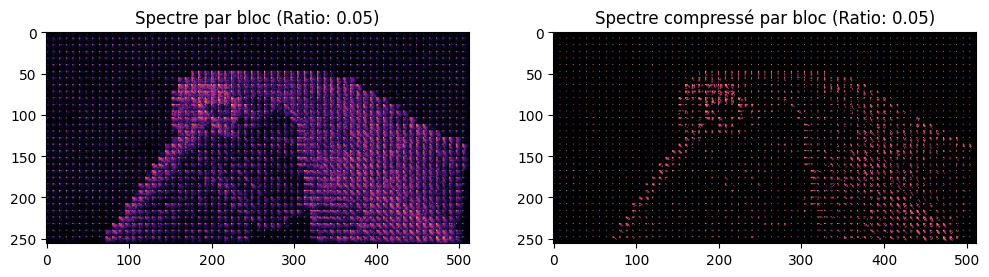
\includegraphics[width=1.15\textwidth]{images/Spectre_DCT.png}
    \caption{Spectre de l'image après application de la transformée en cosinus discrète}
\end{figure}
\begin{figure}[H]
    \centering
    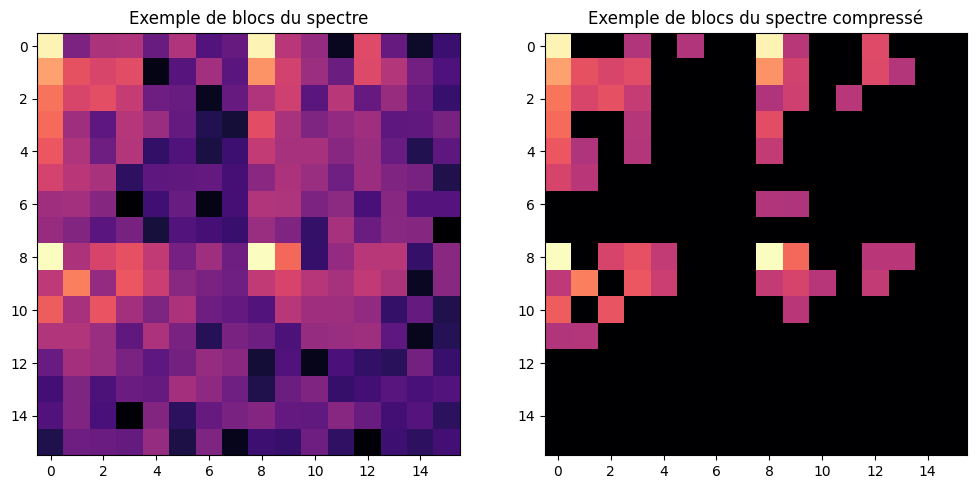
\includegraphics[width=0.65\textwidth]{images/Bloc_DCT.png}
    \caption{Exemple de 4 blocs (8 $\times$ 8) contenus dans le spectre}
\end{figure}
\begin{figure}[H]
    \centering
    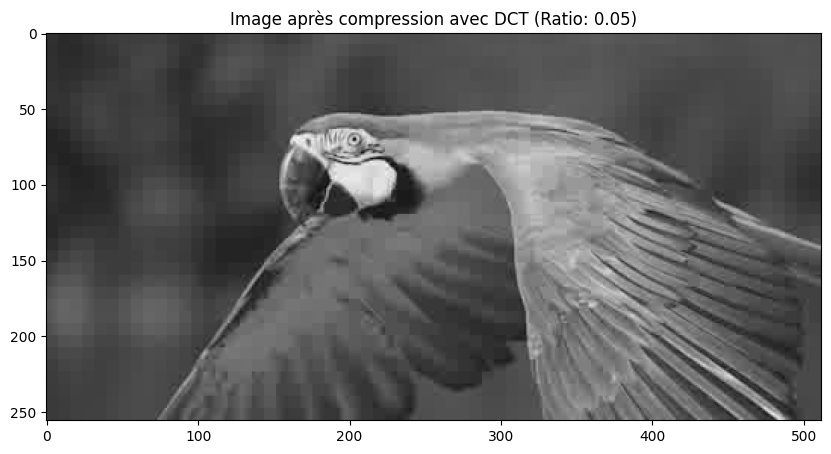
\includegraphics[width=0.75\textwidth]{images/Image_DCT.png}
    \caption{Image finale après application de la DCT et de la compression avec un taux de conservation d'information de 5\%}
\end{figure}
On observe que le fond est plus compressé, d'où les blocs plus visibles, car l'image d'origine comprend un fond  peu détaillé. 
L'objet contenant le plus de détails (ici le perroquet) est peu affecté par la compression.